\chapter{Background}
\vspace{1cm}

Background blah.

\section{File Systems}

The file system is a fundamental abstraction for almost all modern operating
systems. The abstraction allows the operating system and user programs to
interact with a variety of devices and services through a single unified
interface.
The purpose of a specific file system is to implement this common interface for
a particular underlying data store. The exact nature of the data store is not
important to the consumer of the file system's interface. The underlying data
store is commonly a physical storage device such as a hard disk drive (HDD).
However, it is important to note that this is not always the case and there is
no requirement for a file system to manage a physical storage device. File
systems that depend on another file system as their underlying data store are
known as a VFS (virtual file system).

The high level filing cabinet metaphor that is built on the low level interface
provided by a particular file system implementation will be familiar to most
computer users. The metaphor consists of a filing cabinet containing many named
files. These files can contain arbitrary data. However, some of these files may
not contain data themselves but rather other files, and in this case they are
called directories (or folders in some versions of the metaphor). This nesting
of files within directories creates a hierarchical structure where a single
root directory (analogous to the filing cabinet) contains an arbitrarily
deeply nested series of files and directories. The hierarchy of files within
directories can conceptually be arbitrarily deep, but most particular
implementations enforce a limit for simplicity. The filing cabinet metaphor is
also useful in demonstrating that a file or directory can only be contained
within one other directory. Each file or directory (excluding the root
directory) must have one and only one parent in the hierarchy.

In Figure \ref{fig:sample file hierarchy} there are two distinct files named
\texttt{timeline.txt}. It becomes ambiguous to refer to a file only by its name
when this is the case. It is useful to use the steps taken to arrive at a file
or directory to identify it within the file hierarchy. For example, the steps
taken to arrive at \texttt{timeline.txt} would be \texttt{/} then
\texttt{documents} then \texttt{project1} then \texttt{timeline.txt}. This list
of steps is known as a path and can be written as a \texttt{/} delimited list
of the steps taken to reach a file or directory. Using the previous example the
path would be \texttt{/documents/project1/timeline.txt}. As a result of the
single parent rule, each file or directory has a single path that uniquely
identifies it amongst all other files and directories in the hierarchy.
\todo{This is not true when you add links into the equation.}

% Sample file hierarchy figure {{{
\begin{figure}[h]
\centering
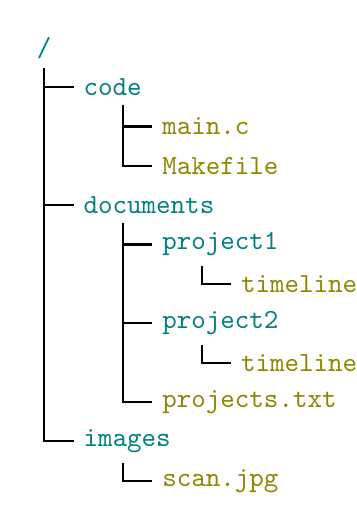
\begin{tikzpicture}[node distance=0.5cm]
    \tikzset{file/.style={rectangle, rounded corners, text=olive, text
        width=1cm, font=\ttfamily}}
    \tikzset{directory/.style={rectangle, rounded corners, text=teal, text
        width=1cm, font=\ttfamily}}
    \tikzset{root directory/.style={rectangle, rounded corners, text=teal,
        font=\ttfamily}}
    \tikzset{arrow/.style=thick}

    \node (root) [root directory] {/};
    \node (code) [directory, below of=root, xshift=1cm] {code};
    \node (mainc) [file, below of=code, xshift=1cm] {main.c};
    \node (makefile) [file, below of=mainc] {Makefile};
    \node (documents) [directory, below of=makefile, xshift=-1cm] {documents};
    \node (project1) [directory, below of=documents, xshift=1cm] {project1};
    \node (timeline1) [file, below of=project1, xshift=1cm] {timeline.txt};
    \node (project2) [directory, below of=timeline1, xshift=-1cm] {project2};
    \node (timeline2) [file, below of=project2, xshift=1cm] {timeline.txt};
    \node (projectstxt) [file, below of=timeline2, xshift=-1cm] {projects.txt};
    \node (images) [directory, below of=projectstxt, xshift=-1cm] {images};
    \node (scanjpg) [file, below of=images, xshift=1cm] {scan.jpg};

    \draw [arrow] (root) |- (code);
    \draw [arrow] (code) |- (mainc);
    \draw [arrow] (code) |- (makefile);
    \draw [arrow] (root) |- (documents);
    \draw [arrow] (documents) |- (project1);
    \draw [arrow] (project1) |- (timeline1);
    \draw [arrow] (documents) |- (project2);
    \draw [arrow] (project2) |- (timeline2);
    \draw [arrow] (documents) |- (projectstxt);
    \draw [arrow] (root) |- (images);
    \draw [arrow] (images) |- (scanjpg);
\end{tikzpicture}
\caption[Sample file hierarchy]{Sample file hierarchy with directories in blue
    and files in green.}
\label{fig:sample file hierarchy}
\end{figure}
% }}}

\subsection{System Calls and the File System}

\todo{
    Talk about how ls makes a system call and the kernel receives it and then
    calls the fuse kernel module who then writes to unix socket which fuser
    (Rust) reads who then calls me. In the general case libFUSE would call the
    libc function mount with fs type 'fuse'. In my case fuser calls fusermount3
    and listens to the returned unix socket for messages from the kernel.
}
